\documentclass[10.5pt,notitlepage]{article}
\usepackage[utf8]{inputenc}
\usepackage{amsthm}
\usepackage{amsmath}
\usepackage{amsfonts}
\usepackage{mathtools}
\usepackage{amsmath,amssymb}       
\usepackage{enumitem}   
\usepackage{enumerate}
\usepackage{verbatim} 
\usepackage{bbm}
\usepackage[backend=biber,style=apa]{biblatex}
\usepackage{csquotes}
\DeclareLanguageMapping{spanish}{spanish-apa}
\urlstyle{same}
\addbibresource{refer.bib}
\usepackage{etoolbox}
\patchcmd{\thebibliography}{\section*{\refname}}{}{}{}
\usepackage{hyperref}
\usepackage{booktabs}
\renewcommand{\qedsymbol}{$\blacksquare$}
\usepackage{makecell}
\usepackage[spanish]{babel}
\decimalpoint
\usepackage[letterpaper]{geometry}
\usepackage{mathrsfs}
\newenvironment{solucion}
  {\begin{proof}[Solución]}
  {\end{proof}}
\pagestyle{plain}
\usepackage{pdflscape}
\usepackage[table, dvipsnames]{xcolor}
\usepackage{longtable}
\usepackage{tikz}
\def\checkmark{\tikz\fill[scale=0.4](0,.35) -- (.25,0) -- (1,.7) -- (.25,.15) -- cycle;} 
\usepackage[bottom]{footmisc}
\usepackage{hyperref}
\usepackage{float}
\usepackage[utf8]{inputenc}
\usepackage{placeins}
\DeclareMathOperator{\Tr}{Tr}
\DeclareMathOperator{\diag}{diag}
\DeclareMathOperator{\argmax}{argmax}
\DeclareMathOperator{\argmin}{argmin}
\newcommand{\PP}{\mathbb{P}}
\newcommand{\Bb}{\mathcal{B}}
\newcommand{\RR}{\mathbb{R}}
\newcommand{\Ff}{\mathcal{F}}
\newcommand{\Ss}{\mathcal{S}}
\newcommand{\Aa}{\mathcal{A}}
\newcommand{\Jj}{\mathcal{J}}
\newcommand{\Cc}{\mathcal{C}}
\newcommand{\oo}{\varnothing}
\newcommand{\ee}{\varepsilon}
\newcommand{\Ee}{\mathcal{E}}
\newcommand{\EE}{\mathbb{E}}
\newcommand{\NN}{\mathbb{N}}
\newcommand{\Pp}{\mathcal{P}}
\newcommand{\Mm}{\mathcal{M}}
\newcommand{\lL}{\mathrm{L}}
\newcommand{\Cov}{\mathrm{Cov}}
\newcommand{\Var}{\mathrm{Var}}
\newcommand{\Ll}{\mathcal{L}}
\newcommand{\xx}{\mathbf{x}}
\newcommand{\abs}[1]{\left\lvert #1 \right\rvert}
\newcommand{\norm}[1]{\left\| #1 \right\|}
\newcommand{\inner}[1]{\left\langle #1 \right\rangle}
\newcommand{\corch}[1]{\left[ #1 \right]}
\newcommand{\kis}[1]{\left\{ #1 \right\}}
\newcommand{\pare}[1]{\left( #1 \right)}
\newcommand{\floor}[1]{\lfloor #1 \rfloor}
\newcommand{\Matrix}[1]{\begin{pmatrix} #1 \end{pmatrix}}

\theoremstyle{plain}

\newtheorem{thm}{Teorema}[section] % reset theorem numbering for each chapter
\newtheorem{defn}[thm]{Definición} % definition numbers are dependent on theorem numbers
\newtheorem{lem}[thm]{Lema} % same for example numbers
\newtheorem{remarkex}{Observación}
\newenvironment{rem}
  {\pushQED{\qed}\renewcommand{\qedsymbol}{$\triangle$}\remarkex}
  {\popQED\endremarkex}

\usepackage{geometry}
\usepackage{mathtools}
\usepackage{enumitem}
\usepackage{framed}
\usepackage{amsthm}
\usepackage{thmtools}
\usepackage{etoolbox}
\usepackage{fancybox}

\newenvironment{myleftbar}{% 
\def\FrameCommand{\hspace{0.6em}\vrule width 2pt\hspace{0.6em}}%
\MakeFramed{\advance\hsize-\width \FrameRestore}}%
{\endMakeFramed}
\declaretheoremstyle[
spaceabove=6pt,
spacebelow=6pt
headfont=\normalfont\bfseries,
headpunct={} ,
headformat={\cornersize*{2pt}\ovalbox{\NAME~\NUMBER\ifstrequal{\NOTE}{}{\relax}{\NOTE}:}},
bodyfont=\normalfont,
]{exobreak}

\declaretheorem[style=exobreak, name=Ejercicio,%
postheadhook=\leavevmode\myleftbar, %
prefoothook = \endmyleftbar]{exo}
\usepackage{graphicx}
\graphicspath{ {images/} }
\title{Tarea 8: Introducción a Ciencia de Datos.}

\author{Rojas Gutiérrez Rodolfo Emmanuel}

\begin{document}
\maketitle
\section{Ejercicios.}
\setcounter{exo}{0}
\begin{exo}

\end{exo}
\begin{solucion}
Para la resolución de este ejercicio, sea \(X \in M_{N \times p}(\RR)\) una matriz de covariables, \(y \in M_{N \times 1}(\RR)\) un vector columna de variables independientes y \(f_{\lambda}\) la función \(f_{\lambda}: M_{p \times 1}(\RR) \mapsto \RR_{+}\) con regla de correspondencia:
\begin{align}\label{lab.1}
    f_{\lambda}(\beta) =\frac{1}{2N}\norm{y - X\beta}^2 +\lambda \norm{\beta}_{1}, 
\end{align}
donde, los símbolos \(\norm{}\) y \(\norm{}_1\) denotan de manera respectiva, la norma euclidiana en \(\RR^{N}\) y la norma \(l_1\) en \(\RR^{p}\). Ahora, observe que gracias a la relación que guardan entre si, la norma euclidiana en \(\RR^{N}\) y el producto interno en \(\RR^N\), se tiene para cada \(\beta \in M_{p \times 1}(\RR)\) que
\begin{align}\label{lab.2}
    \norm{y - X\beta}^2 = \norm{y}^2 + \norm{X \beta}^2 - \inner{y, X\beta}. 
\end{align}
Luego, recordando que para \(\beta \in M_{p \times 1}(\RR)\), el producto \(X \beta\) puede expresarse como una combinación lineal de la columnas de \(X\), de la siguiente forma:
\begin{align*}
    X\beta  = \sum_{j = 1}^{n}\beta_{j}X_{j} 
\end{align*}
donde, para \(j \in \kis{1, \hdots, p}\) se tiene que \(X_{j}\) denota a la \(j\)-ésima columna de \(X\), mientras que, \(\beta_{j}\) representa a la \(j\)-esima entrada del vector columna \(\beta\). Así, al sustituir la expresión anterior en la igualdad en \eqref{lab.2}, se obtiene que:
\begin{align}
     \norm{y - X\beta}^2 &=  \norm{y}^2 + \norm{X \beta}^2 - 2\inner{y, \sum_{j = 1}^{n}\beta_{j}X_{j}} \nonumber\\  
                         &=  \norm{y}^2 + \norm{X \beta}^2 - 2\sum_{j = 1}^{n}\beta_{j}\inner{y,X_{j}} \label{lab.3},
\end{align}
donde, la segunda igualdad se debe a la bilinealidad del producto interno. Luego, dado que para cada \(j \in \kis{1, \hdots, p}\) se tiene que
\[
\beta_{j}\inner{y,X_{j}} \leq \abs{\beta_{j}\inner{y,X_{j}}} \leq \abs{\beta_j} \max_{j \in \kis{1,\hdots,p}}\abs{\inner{y,X_{j}}}.
\]
entonces, se sigue que
\[
-\beta_{j}\inner{y,X_{j}} \geq -\abs{\beta_j} \max_{j \in \kis{1,\hdots,p}}\abs{\inner{y,X_{j}}}, \text{ para cada } j \in \kis{1, \hdots,p}.
\]
Así, de la desigualdad anterior y de la igualdad en \eqref{lab.3}, se deduce que 
\begin{align*}
    \norm{y - X\beta}^2 &\geq \norm{y}^2 + \norm{X \beta}^2  - 2\corch{\sum_{j = 1}^{p}\max_{j \in \kis{1,\hdots,p}}\abs{\inner{y,X_{j}}}\abs{\beta_j}}.\\
                        &= \norm{y}^2 + \norm{X \beta}^2  - 2\max_{j \in \kis{1,\hdots,p}}\abs{\inner{y,X_{j}}}\corch{\sum_{j = 1}^{p}\abs{\beta_j}}.
\end{align*}
Lo que implica que 
\begin{align*}
\frac{1}{2N}\norm{y - X\beta}^2 &\geq \frac{1}{2N}\corch{\norm{y}^2 + \norm{X \beta}^2 -2\max_{j \in \kis{1,\hdots,p}}\abs{\inner{y,X_{j}}}\corch{\sum_{j = 1}^{p}\abs{\beta_j}}} \nonumber\\ 
                                &=\frac{1}{2N}\corch{\norm{y}^2 + \norm{X \beta}^2 -2\max_{j \in \kis{1,\hdots,p}}\abs{\inner{y,X_{j}}}\norm{\beta}_1}.    
\end{align*}
donde, la última desigualdad se debe a que \(\beta = \Matrix{\beta_1 & \hdots & \beta_p}'\). De este modo, por la desigualdad anterior y la igualdad en \eqref{lab.1}, se obtiene que
\begin{align*}
f_{\lambda}(\beta) &\geq  \frac{1}{2N}\corch{\norm{y}^2 + \norm{X \beta}^2} -\frac{2}{2N}\max_{j \in \kis{1,\hdots,p}}\abs{\inner{y,X_{j}}}\norm{\beta}_1 + \lambda \norm{\beta}_1\\
                   &= \frac{1}{2N}\norm{y}^2 + \frac{1}{2N}\norm{X \beta}^2 + \pare{\lambda  -\frac{1}{N}\max_{j \in \kis{1,\hdots,p}}\abs{\inner{y,X_{j}}}}\norm{\beta}_1\\ 
                   &\geq  \frac{1}{2N}\norm{y}^2 + \pare{\lambda  -\frac{1}{N}\max_{j \in \kis{1,\hdots,p}}\abs{\inner{y,X_{j}}}}\norm{\beta}_1.
\end{align*}
donde, la segunda desigualdad se debe a que \((2N)^{-1}\norm{X \beta}^2 \geq 0\), pues, es la norma euclidiana de \(X \beta\). Finalmente, de la última desigualdad se deduce que si \(\lambda \geq N^{-1}\max_{j \in \kis{1,\hdots,p}}\abs{\inner{y,X_{j}}}\), entonces: 
\begin{align}\label{lab.6}
f_{\lambda}(\beta) &\geq  \frac{1}{2N}\norm{y}^2.
\end{align}
pues, en este caso el término \( \pare{\lambda  - N^{-1}\max_{j \in \kis{1,\hdots,p}}\abs{\inner{y,X_{j}}}}\norm{\beta}_1\) es mayor o igual a cero, ya que, \(\norm{\beta}_1\) es también mayor o igual a cero. Ahora, note que \[\frac{1}{2N}\norm{y}^2=\frac{1}{2N}\norm{y - X 0}^2 + \lambda\norm{0}_1  = f_{\lambda}(0).\]
De este modo, la desigualdad en \eqref{lab.6} puede escribirse como 
\[
f_{\lambda}(\beta) \geq f_{\lambda}(0), \text{ siempre que } \lambda \geq \frac{1}{N}\max_{j \in \kis{1,\hdots,p}}\abs{\inner{y,X_{j}}}.
\]
Así, de la arbitrariedad de \(\beta \in M_{p \times 1}(\RR)\), se sigue que
\[
f_{\lambda}(\beta) \geq f_{\lambda}(0), \text{ para cada } \beta \in M_{p \times 1}(\RR) \text{ siempre que } \lambda \geq \frac{1}{N}\max_{j \in \kis{1,\hdots,p}}\abs{\inner{y,X_{j}}}.
\]
Por lo que, de lo anterior es posible concluir que 
\[
\min_{\beta \in M_{p \times 1}(\RR)}f_{\lambda}(\beta) = f_{\lambda}(0), \text{ siempre que } \lambda \geq \frac{1}{N}\max_{j \in \kis{1,\hdots,p}}\abs{\inner{y,X_{j}}}
\]
y, que 
\[
\argmin_{\beta \in M_{p \times 1}(\RR)}f_{\lambda}(\beta) = 0, \text{ siempre que } \lambda \geq \frac{1}{N}\max_{j \in \kis{1,\hdots,p}}\abs{\inner{y,X_{j}}}.
\]
Por lo cual, de las dos igualdades anteriores, se concluye que es posible tomar el valor \(\lambda_{\max}\) solicitado como:
\[
\lambda_{\max} = \frac{1}{N}\max_{j \in \kis{1,\hdots,p}}\abs{\inner{y,X_{j}}}.
\]
Finalmente, no se sabe si existe una forma analítica cerrada para \(\lambda_{\min}\), no obstante, lo que si sabe es que al elegir \(\lambda = 0\), las estimaciones Lasso para el vector de coeficientes, coinciden con las hechas por mínimo cuadrados. Más aún, bajo la normalidad de los términos de error, se tiene que el estimador de mínimos cuadrados para \(\beta\), posee una distribución Gaussiana multivariada, por lo que, en este caso la probabilidad de que alguna de sus entradas sea igual a cero, es exactamente cero. Basados en esto, se piensa que el valor de \(\lambda_{\min}\) debe elegirse muy cercano a cero, por ejemplo, \(\lambda_{\min} = 10^{-3}\), con lo que. las estimaciones Lasso y de mínimos cuadrados deberían ser casi iguales y se esperaría que ningún termino estimado fuese nulo.

\end{solucion}
%%%%%%%%%%%%%%%%%%%%%%%%%%%%%%%%%%%%%%%%%%%%%%%%%%%%%%%%%%%%%%%%%%%%%%%%%%%%%%%%%%%%%%%%%%%%%%%%%%%%%%%%%%%%%%%%%%%%%%%%%%%%%%%%%%%%%%%%%%%%%%%%%%%%%%%%%%%%%%%%%%%%%
\begin{exo}

\end{exo}
\begin{solucion}
Primeramente, el conjunto de datos Prostate se presenta a continuación:\footnote{Los datos al completo, pueden ser consultados en \(R\).}

\begin{table}[H]
        \centering
\scalebox{0.7}{        
        \begin{tabular}{@{}l@{\hskip 0.3in}r@{\hskip 0.3in}r@{\hskip 0.3in}r@{\hskip 0.3in}r@{\hskip 0.3in}r@{\hskip 0.3in}r@{\hskip 0.3in}r@{\hskip 0.3in}r@{}}
        \toprule
        \(lpsa\)& \(pgg45\)& \(gleason\)&\(lcp\)&\(svi\)&\(lbph\)&\(age\) &\(lweight\)& lcavol\\ 
        \midrule          
          -0.431&     0&       6& -1.386 &  0& -1.386&  50&   2.769& -0.580\\
          -0.163&     0&       6& -1.386 &  0& -1.386&  58&   3.320& -0.994\\
          -0.163&    20&       7& -1.386 &  0& -1.386&  74&   2.691& -0.511\\
          \vdots&    \vdots&   \vdots&  \vdots& \vdots&\vdots&\vdots&\vdots&\vdots\\
           5.143&    10&       7&  2.464&   1& -1.386&  52&   3.396&  2.907\\
           5.478&    80&       7&  1.558&   1&  1.558&  68&   3.774&  2.883\\
           5.583&    20&       7&  2.904&   1&  0.438&  68&   3.975&  3.472\\
        \end{tabular}
}        
        \caption{Datos Prostate provenientes de la librería \(lasso2\) de \(R\).}
        \label{tab:1}
\end{table}

Este conjunto de datos, forma parte de un estudio sobre la relación que existe entre el antígeno específico de prostata (lpsa) y otras variables clínicas. El objetivo de este ejercicio, será ajustar un modelo de regresión lineal para predecir lpsa en función del resto de variables, para luego comparar las variables seleccionadas
con las que selecciona un método 'stepwise' hacia atrás. Para ello, sea \(y\in M_{97 \times 1}(\RR)\) el vector columna de datos, cuya \(i\)-esima entrada corresponde a la \(i\)-esima entrada de la primer columna en el Cuadro \ref{tab:1}, menos la media muestral de esta primer columna, en notación:   
\[
y_i = lpsa_i  - \overline{lpsa}, \text{ con } i \in \kis{1, \hdots, 97}.
\]
Y, sea \(X\in M_{97 \times 8}(\RR)\) la matriz de datos, cuyas columnas coinciden con las columnas \(2\) a \(9\) de la tabla de datos en \ref{tab:1} y denote por \(X^{(c)}\in M_{97 \times 8}(\RR)\), a la versión de \(X\) cuyas columnas han sido centradas y escaladas para tener norma \(N = 97\).\footnote{Dado que el objetivo del modelo es únicamente predictivo, estos cambios de escala en las variables predictoras, como se mencionó en clase, no resultan relevantes.} Entonces, el objetivo de este ejercicio sera ajustar un modelo de regresión lineal de la forma 
\begin{equation}\label{lab.mode}
    y = X^{(c)}\beta  + \ee,
\end{equation}
donde, \(\ee\) es un vector de términos de error que se supondrán no correlacionados, de media cero y varianza homocedástica \(\sigma^2 >0\), mientras que, \(\beta = \Matrix{\beta_1 & \hdots & \beta_8}'\in M_{8 \times 1}(\RR)\) es un vector de coeficientes lineales. No obstante, puede que no todas las covariables en \(X^{(c)}\) sean realmente significativas para el modelo,\footnote{O que incluirlas a todas cause un sobre-ajuste, o traiga consigo problemas de multicolinealidad.} por lo que, una forma de seleccionar que covariables serán incluidas en el mismo es mediante regresión Lasso. Por ende, el primer paso en este ejercicio, será el ajustar un modelo de regresión Lasso al minimizar, la función   
\[
f_{\lambda}(\beta) = \frac{1}{N}\norm{y - X^{(c)}\beta}^2 + \lambda\norm{\beta}_1, \text{ con } \beta = \Matrix{\beta_1 & \hdots & \beta_8}'\in M_{8 \times 1}(\RR),
\]
para algún \(\lambda > 0\), el cual será elegido mediante validación cruzada de tal suerte que se minimice el error cuadrático promedio muestral, al seleccionar dicho \(\lambda\) como parámetro de penalización para el modelo a ajustar mediante regresión Lasso. Con esto en mente, se hizo uso de la librería \(glmnet\) de \(R\), para explorar las estimaciones para el vector de parámetros \(\beta\), obtenidas mediante regresión Lasso, al variar el valor del parámetro \(\lambda\) en un cierto rango. Ahora, para determinar el rango de posibles valores para el parámetro \(\lambda\), se hizo uso de lo probado en el inciso \textbf{a)} de este ejercicio, por ende, se calculo el valor:
\[
\lambda_{\max} = \frac{1}{N}\max_{1 \leq j \leq 8}\abs{\inner{y,X^{(c)}_{j}}} \approx 0.95065,
\]
donde, para \(j \in \kis{1, \hdots, 8}\), se tiene que \(X^{(c)}_{j}\) representa a la \(j\)-ésima columna de \(X^{(c)}\). De este modo, se eligió variar el parámetro \(\lambda\) en el intervalo \([\lambda_{\min}, \lambda_{\max}]\), donde, \(\lambda_{min} = 10^{-2}\) se eligió muy cercano a cero, pues, con esta elección de valores para \(\lambda_{\min}\) y \(\lambda_{\max}\) se esperaría, por lo hecho en el inciso \textbf{a),} que existiesen valores de \(\lambda\) en \([\lambda_{\min}, \lambda_{\max}]\) para los que se tuvieran estimaciones Lasso para los coeficientes de \(\beta\), desde el caso en el que todas estas estimaciones son cero, hasta el caso en el que ninguna de las mismas es cero. Habiendo determinado el rango de valores a tomar en cuenta para la elección del parámetro \(\lambda\), se empleo la función \(glmnet\) para obtener la gráfica presentada en la Figura \ref{fig:1}. Observe que, en la parte superior de dicha gráfica, se puede observar el número de covariables cuyo coeficiente de pendiente \(\beta_j\) asociado, tiene una estimación distinta de cero para el valor de \(\lambda\) indicado en el eje \(x\). Note que, en esta gráfica se corrobora que al considerar valores para \(\lambda\) en el intervalo \([\lambda_{\min}, \lambda_{\max}]\), se esta considerando modelos que arrojan desde \(0\) hasta \(8\) de las estimaciones para los componentes de \(\beta\), distintas de cero. 
\begin{figure}[htb]
    \centering
    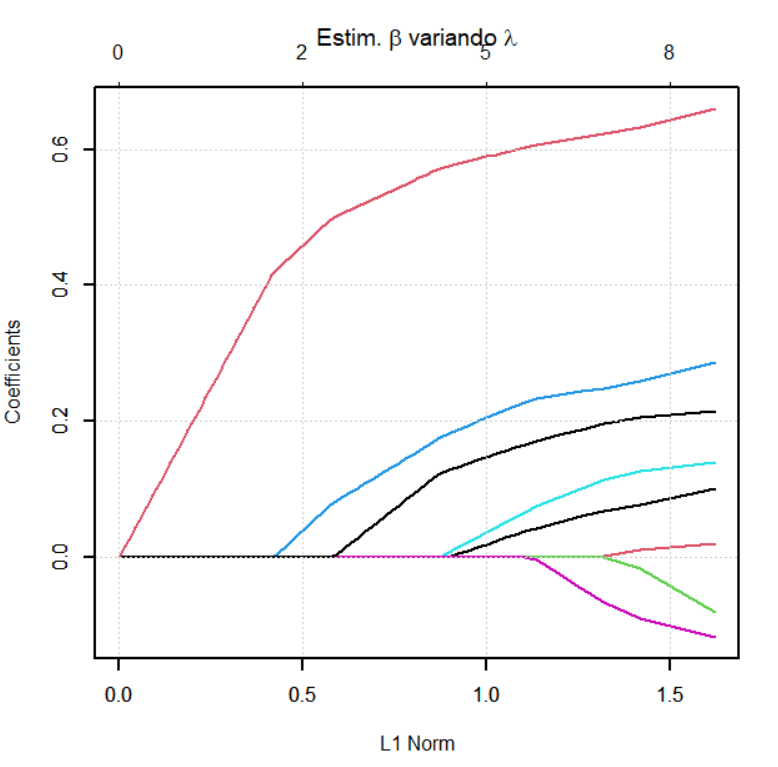
\includegraphics[scale = 0.4]{Esims.png}
    \caption{Estimaciones para el vector de coeficientes \(\beta\) obtenidas por Regresión Lasso, al variar el parámetro de penalización \(\lambda\) en el intervalo \([\lambda_{\min},\lambda_{\max}]\).}
    \label{fig:1}
\end{figure}

Ahora, para seleccionar el valor adecuado para \(\lambda\) dentro del intervalo \([\lambda_{\min}, \lambda_{\max}]\), se hizo uso de la función \(cv.glmnet\) la cual emplea la técnica de \(n\)-fold cross validation, para encontrar el valor de \(\lambda\) que produce el menor Error cuadrático promedio posible. De manera breve, el numero \(n\) en el nombre de esta metodología, denota el número de grupos en los que se parte de manera aleatoria el conjunto de datos originales, para llevar a cabo el ajuste del modelo Lasso con algún valor de \(\lambda\) especificado, usando para dicho ajuste todos los grupos de datos formados salvo uno,\footnote{A los datos usados para el ajuste, se les conoce como datos de entrenamiento. Mientras que, los datos que se excluyen al realizar el ajuste, se conocen como datos de prueba.} para luego, probar que tan bueno es el ajuste del modelo en el grupo que quedo fuera, obteniendo una estimación del error cuadrático que comete el modelo, al hacer predicciones en este último grupo. Esto último, se realiza dejando fuera cada uno de los grupos en que se separo el conjunto, con lo que, se obtien un conjunto de estimaciones del error cuadrático promedio (ECP), que tiene el modelo ajustado usando el parámetro de penalización \(\lambda\). Así, al promediar todos estas estimaciones del ECP, se obtiene una única estimación para el ECP que comete el modelo, cuando se elige por parámetro de penalización a \(\lambda\). Así, para elegir el parámetro de penalización a usar, la idea fue llevar a cabo este algoritmo aplicándolo a los valores en el intervalo \([\lambda_{\min}, \lambda_{\max}]\) seleccionados y, elegir por parámetro de penalización para el modelo final, a aquel valor de \(\lambda\) asociado a la estimación más pequeña del ECP. Todo esto, como ya menciono con anterioridad, puede llevarse a acabo haciendo uso de la función \(cv.glmnet\). Cabe destacar que, el paquete \(glmnet\) recomienda hacer uso del algoritmo \(10\)-fold CV, no obstante, en Modelos Estadísticos \(I\) se vio que en el caso de Regresión Ridge, es preferible usar el algorito Leave-One-Out  CV,\footnote{Aquel que forma \(N\) grupos.} por ende, se llevaron ambos algoritmos a cabo. Ahora, entre los resultados producidos con \(cv.glmnet\), se obtiene el valor de \(\lambda\) con el cual se consigue el menor error cuadrático promedio posible, por lo que, es importante mencionar que en este caso, se tiene que el valor de \(\lambda\) obtenido al usar el algoritmo \(10\)-fold CV, es exactamente igual al valor de \(\lambda\) obtenido mediante el algoritmo Leave-One-Out CV y que, dicho valor de \(\lambda\), el cual se denotará por \(\lambda^*\), esta dado por:
\[
\lambda^* = 0.029.
\]
Lo anterior, puede corroborarse de manera visual al observar la gráfica en la Figura \ref{fig:2}.\footnote{Las cual, también se ha producido al emplear la función \(cv.glmnet\).} Pues, al lado izquierdo de dicho gráfico, puede ver una gráfica del \(\log(\lambda)\) contra el ECP estimado mediante el uso del algoritmo \(10\)-fold CV, cuando se usa el parámetro de penalización \(\lambda\). Mientras que, de lado derecho se puede observar gráfica del \(\log(\lambda)\) contra el ECP estimado mediante el uso del algoritmo Leave-One-Out CV, cuando se usa el parámetro de penalización \(\lambda\). En ambas gráficas, la primer linea vertical punteada que aparece de izquierda a derecha, se encuentra remarcada a la altura \(x  =\log(\lambda^*)\). Así, se corrobora de manera visual, que el menor ECP estimado sea mediante \(10\)-fold CV o mediante Leave-One-Out CV, se obtiene al tomar como parámetro de penalización a \(\lambda^*\). 
\begin{figure}[htb]
    \centering
    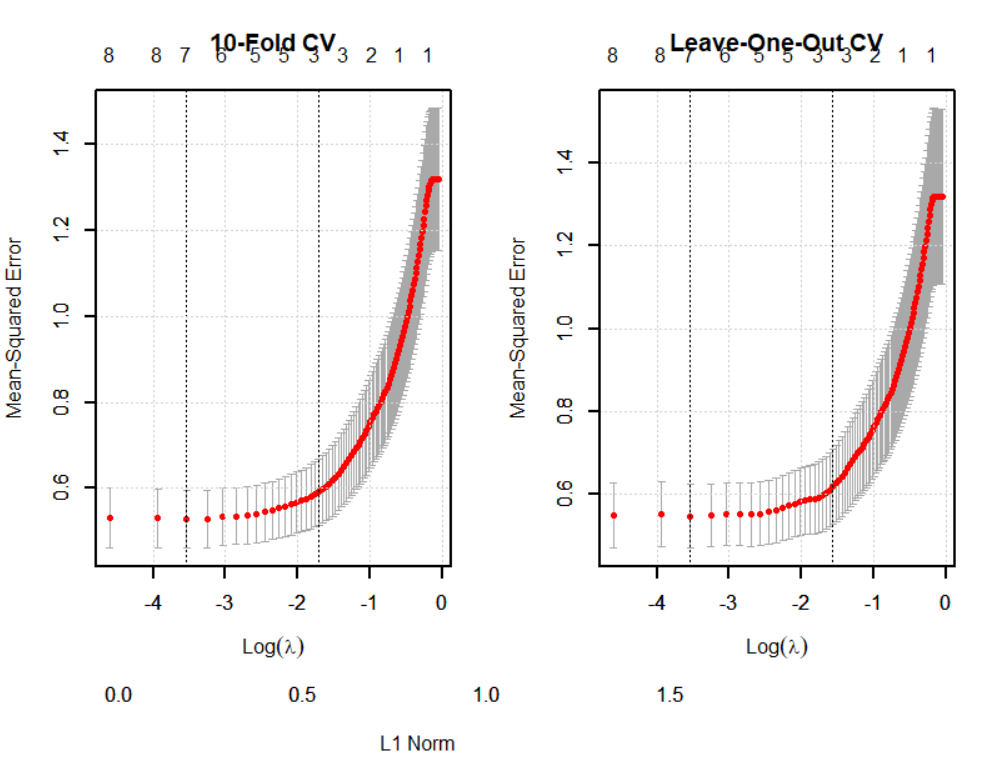
\includegraphics[scale = 0.5]{CV.png}
    \caption{Gráfica de ECP estimado vs logaritmo del parámetro de penalización. Valores del parámetro de penalización en el intervalo \([\lambda_{\min}, \lambda_{\max}]\).}
    \label{fig:2}
\end{figure}
Ahora, nombre de manera respectiva a las columnas de \(X^{(c)}\), como las últimas \(8\) columnas de la tabla de datos en el Cuadro \ref{tab:1}, añadiendo el prefijo \(sc\) a los nombres de estas últimas \(8\) columnas, como una abreviación para hacer referencia al centrado y escalado hecho para obtener \(X^{(c)}\). A modo de ejemplo de esto, la primer columna de \(X^{(c)}\) se identificará con el nombre \(scpgg45\). De este modo, para \(i \in \kis{1,\hdots,8}\), note que \(\beta_i\) la \(i\)-ésima componente de \(\beta\), es el parámetro de pendiente en el modelo en \eqref{lab.1} asociado a la variable en la columna \(i\), de la matriz \(X^{(c)}\). Con esto en mente, se presenta en el Cuadro \ref{tab:2} los coeficientes estimados mediante el algoritmo Lasso, cuando se utiliza como parámetro de penalización a \(\lambda^*\). Puede notar que, mediante la técnica de regresión Lasso se han incluido todas las variables salvo la variable en la columna \(3\), \(sclcp\), de la matriz \(X^{(c)}\).  
\begin{table}[htb]
    \centering
        \centering
        \begin{tabular}{@{}l@{\hskip 0.3in}r@{\hskip 0.3in}r@{}}
        \toprule
Nombre columna& Coef & Estimación Lasso\\        
\midrule        
scpgg45    &\(\beta_1\)& 0.0689\\
scgleason  &\(\beta_2\)& 0.0030\\
sclcp      &\(\beta_3\)&0      \\ 
scsvi      &\(\beta_4\)& 0.2495\\
sclbph     &\(\beta_5\)& 0.1136\\
scage      &\(\beta_6\)&-0.0658\\
sclweight  &\(\beta_7\)& 0.1971\\
sclcavol   &\(\beta_8\)& 0.6223\\
        \end{tabular}
    \caption{Caption}
    \label{tab:2}
\end{table}
Por otro lado, otra técnica de selección de modelos es el algoritmo de selección automatizada 'stepwize' hacia atrás. Este algoritmo, consiste en ajustar el modelo en \eqref{lab.mode} mediante mínimos cuadrados,\footnote{Es decir, el modelo que contempla todas las variables.} para luego ver el efecto que tiene en el modelo el quitar una a una, cada una de las variables en el mismo y ajustar con las covariables restantes, un modelo de regresión mediante mínimos cuadrados. Luego, si el quitar una de estas covariables, trae consigo el menor \(AIC\) en el modelo de regresión ajustado sin la misma, donde el término menor debe entenderse respecto a los \(AIC\) tanto del modelo completo, como de los modelos en los que no se considera a las otras variables, entonces dicha covariable es removida del modelo, lo que da paso a un modelo reducido al cual se le vuelve a aplicar esta misma técnica. El algoritmo concluye cuando el quitar covariables del modelo no trae consigo un menor \(AIC\) que el \(AIC\) del modelo más completo. Ahora, para aplicar este algoritmo puede usarse la función \(step\) de \(R\), especificando el argumento \(direction = 'backward'\). Haciendo esto, se obtienen todos y cada uno de los pasos del algoritmo, necesarios para llegar del completo modelo a aquel en el cual ya no hay mejorías en el \(AIC\), no obstante, en nuestro caso por cuestiones de espacio solo se pondrá la primer y última tablas producidas por \(step\),\footnote{Para ver este análisis en su totalidad puede ir al script adjunto.} dichas tablas se presentan de manera respectiva en los Cuadros \ref{tab:3} y \ref{tab:4}. Ahora, fije su atención en la columna \(AIC\) del Cuadro \ref{tab:3}, en ella se muestra el \(AIC\) resultante al omitir del modelo completo la variable especificada en la columna Var. omitida, como puede ver el \(AIC\) del modelo completo es \(-60.322\) y al remover la covariable \(scgleason\), se obtiene el \(AIC\) más pequeño posible, por lo que, esta es la primer covariable removida del modelo por el algoritmo. Finalmente, en la columna \(AIC\) en el Cuadro \ref{tab:4}, puede ver que el \(AIC\) más pequeño se obtiene cuando no se remueve ninguna covariable al modelo que considera únicamente a las covariables \(\kis{\text{scage,sclbph,sclweight,scsvi,sclcavol}}\), es decir, aquel en el que los coeficientes en \(\beta\) que no son cero, están dados por \(\kis{\beta_4,\beta_5,\beta_6,\beta_7,\beta_8}\).  
\begin{table}[htb]
    \centering
        \centering
        \begin{tabular}{@{}l@{\hskip 0.3in}r@{\hskip 0.3in}r@{\hskip 0.3in}r@{\hskip 0.3in}r@{}}
        \toprule
Var. omitida& Df& Sum of Sq&\(RSS\)&\(AIC\) \\  
        \midrule        
- scgleason & 1&    0.0412 &44.204& -62.231\\
- scpgg45  &  1&    0.5258 &44.689& -61.174\\
- sclcp    &  1&    0.6740 &44.837& -60.852\\
\(<\)ninguna\(>\)  &    -&   -        &44.163& -60.322\\
- scscage  &  1&    1.5503& 45.713& -58.975\\
- sclbph   &  1&    1.6836& 45.847& -58.693\\
- sclweight&  1&    3.5860& 47.749& -54.749\\
- scsvi    &  1&    4.9355& 49.099& -52.045\\
- sclcavol&   1&   22.3722& 66.535& -22.567\\
        \end{tabular}
    \caption{Primer paso del algoritmo 'stepwize' hacia atrás: El cual consiste en quitar variables al modelo original.}
    \label{tab:3}
\end{table}
\begin{table}[htb]
    \centering
        \centering
        \begin{tabular}{@{}l@{\hskip 0.3in}r@{\hskip 0.3in}r@{\hskip 0.3in}r@{\hskip 0.3in}r@{}}
        \toprule
Var. omitida& Df& Sum of Sq&    RSS&     AIC\\  
        \midrule        
\(<\)ninguna\(>\) &    -    &   -    & 45.526& -63.374\\
- scage  &    1   & 0.9593& 46.485& -63.352\\
- sclbph &    1   & 1.8568& 47.382& -61.497\\
- sclweight&  1   & 3.2250& 48.751& -58.735\\
- scsvi    &  1   & 5.9517& 51.477& -53.456\\
- sclcavol &  1   &28.7666& 74.292& -17.87\\
        \end{tabular}
    \caption{Último paso del algoritmo 'stepwize' hacia atrás.}
    \label{tab:4}
\end{table}
Finalmente, se ajusto con ayuda de la función \(lm\) de \(R\), el modelo sugerido por el método 'stepwize' hacia atrás. Un resumen del ajuste anterior, puede verse en el Cuadro \ref{tab:5}. Ahora, observando los Cuadros \ref{tab:2} y \ref{tab:5}, se puede ver que ambos métodos de selección de variables, dejan fuera a la variable \(sclcp\), más aún, las otras dos variables que deja fuera el método de selección 'stepwize' hacia atrás, tienen coeficientes estimados por Lasso muy cercanos a cero, mientras que, el resto de coeficientes se han estimado con el mismo signo por ambos métodos y las estimaciones resultan relativamente similares. Finalmente, por cuestiones de parsimonia del modelo y dado que como se comento previamente, las estimaciones por regresión Lasso para los coeficientes de scpgg45 y scgleason son cercanas a cero, elegiría el modelo seleccionado mediante el método 'stepwize' hacía atrás. 
\begin{table}[H]
        \centering
        \begin{tabular}{@{}l@{\hskip 0.3in}r@{\hskip 0.3in}r@{\hskip 0.3in}r@{\hskip 0.3in}r@{\hskip 0.3in}r@{}}
            \toprule
        Nombre Col&Coeficiente& Estimación & \(t\)-valor& \(p\)-valor \\
            \midrule
scpgg45    &\(\beta_1\)& 0 & -&-\\
scgleason  &\(\beta_2\)& 0 & -&-\\
sclcp      &\(\beta_3\)&0  &-&-    \\             
scsvi  & \(\beta_{4}\)  & 0.29693   &3.468 &0.000799 \\
sclbph &\(\beta_{5}\)  & 0.16142   &1.937 &0.055803   \\
scage  &\(\beta_{6}\) &-0.11030   &-1.392 &0.167188    \\
sclweight&\(\beta_{7}\)& 0.20933   &2.553 &0.012329   \\
sclcavol&\(\beta_{8}\)& 0.66320   &7.624 &2.16\(\cdot 10^{-11}\)\\
            \bottomrule
        \end{tabular}
        \caption{Estimaciones para el modelo ajustado haciendo uso de la función \(step\).}
        \label{tab:5}
\end{table}


\end{solucion}
\end{document}
 